\documentclass[10pt,french]{book}
\input preambule_2013

\newcounter{exoc}
\newenvironment{exoc}[1]{%
  \refstepcounter{exoc}\textbf{Exercice \theexoc} :\hfill {\textbf{(#1)}}\par
  \medskip}%
{\medskip}

\pagestyle{empty}

\newcommand\Kdo[1][1em]{$
\includegraphics[width=10pt]{kdo.eps}\hspace{#1}$}
\newcommand\Red[1][1em]{$\includegraphics[width=10pt]{bc-crayon}\hspace{#1}$}

\begin{document}

\begin{center}
\begin{tabularx}{\textwidth}{|>\centering m{2.5cm}|>\centering X|>{\centering\arraybackslash} m{2.5cm}|}
	\hline
		\seconde 7 &  Mardi 21 janvier \np{2013} & \textbf{Variations de fonctions} \\
	\hline
		\multicolumn{3}{|c|}{\bsc{Contrôle de mathématiques}} \\
	\hline
        \multicolumn{1}{|r}{\bsc{Nom}:} & \multicolumn{2}{l|}{} \\
		\multicolumn{1}{|r}{Prénom:} & \multicolumn{2}{l|}{} \\
	\hline
        \multicolumn{3}{|l|}{\bfseries Note et observations :} \\[1cm]
    \hline
\end{tabularx}\medskip

{\itshape
\small
Le barème est indicatif. Répondre aux questions \textbf{par des phrases}.\par
{\bfseries Pour les questions \Red[0pt], des points sont attribués à la qualité et la précision de la rédaction !}\par
Les questions \Kdo[0pt] doivent absolument être réussie.
}
\end{center}



\begin{exoc}{3x1 + 1 + 1 = 5 points}
La fonction $g$ est définie pour tout $x \in \R$ par $g(x) = x^2 - 2x + 4.$

\begin{enumerate}
    \item En détaillant les étapes, calculer :
    \begin{enumerate}
        \item $g(-1)$
        \item $g(0)$
        \item $g(3)$.
    \end{enumerate}
    \item Paulette affirme que $g$ est croissante sur l'intervalle $\intervalleff{-1}{0}$.\par \Red Que peut-on dire de l'affirmation de Paulette ? Pourquoi ?
    \item Paulo affirme que $g$ est croissante sur l'intervalle $\intervalleff{0}{3}$.\par \Red Que peut-on dire de l'affirmation de Paulo ? Pourquoi ?
\end{enumerate}

\end{exoc}\[*\]

\begin{exoc}{0,5 + 5x1 + 1,5 = 7 points}
    Dans un repère \OIJ, La fonction $f$ est définie sur son ensemble de définition $\calig D_f$ par sa courbe représentative $\calig C_f$ :
    
    \begin{center}
        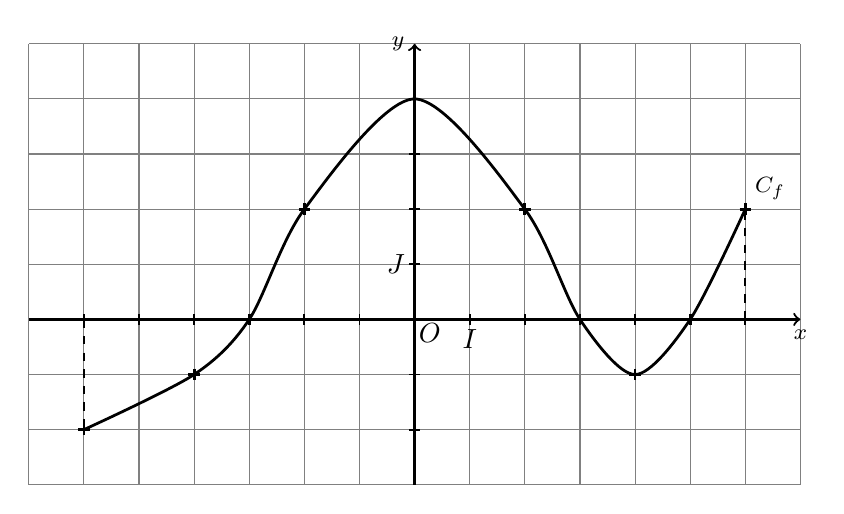
\begin{tikzpicture}[scale=0.7]
            \draw[gray] (-7,-3)grid(7,5);
            \draw[thick,->] (-7,0)--(7,0)node[below] {\footnotesize $x$};
            \draw[thick,->] (0,-3)--(0,5)node[left] {\footnotesize $y$};
            \draw[line width=1pt] plot[smooth=200,mark=+,mark options={scale =1.5}] coordinates{(-6,-2)(-4,-1)(-3,0)(-2,2)(0,4)(2,2)(3,0)(4,-1)(5,0)(6,2)};
            \draw (6,2) node[above right]{\footnotesize $\calig C_f$};
            \coordinate (O) at (0,0); \draw (O) node[below right = -2pt] {$O$};
            \coordinate (I) at (1,0); \draw (I) node[below] {$I$}; \foreach \x in {-6,...,6}  \draw[line width=0.7pt] (\x,-0.1)--(\x,0.1);
            \coordinate (J) at (0,1); \draw (J) node[left] {$J$}; \foreach \x in {-2,...,4} \draw[line width=0.7pt] (-0.1,\x)--(0.1,\x);
            \draw[line width=0.7pt,dashed] (6,0)--(6,2);
            \draw[line width=0.7pt,dashed] (-6,0)--(-6,-2);
        \end{tikzpicture}
    \end{center}
    
\begin{enumerate}
    \item À l'aide du graphique :
    \begin{enumerate}
        \item \Kdo Déterminer $\calig D_f$.
        \item \Kdo Déterminer le maximum $M$ de la fonction $f$. Pour quelle valeur de $x$ est-il atteint ?
        \item \Kdo Déterminer le minimum $m$ de la fonction $f$. Pour quelle valeur de $x$ est-il atteint ?
        \item \Red Résoudre l'équation $f(x) = 2$.
        \item \Red Résoudre l'inéquation $f(x) \geqslant -1$.
        \item \Red Résoudre l'inéquation $f(x) < 0$.
    \end{enumerate}
    \item \Kdo Dresser le tableau de variations de $f$.
\end{enumerate}
\end{exoc}

\begin{center}
\textbf{Tourner la page pour le dernier exercice !}
\end{center}\clearpage

\begin{exoc}{0,5 + 0,5 + 4x1 + 2x1,5 = 8 points}
    $h$ est la fonction définie sur l'intervalle $\calig D_h$ par le tableau de variations ci-dessous.

\begin{center}
    \begin{tikzpicture}
        \tkzTabInit[nocadre,espcl=1.75,lgt=2.5]{$x$/0.75,Variations\\ de $h$/1.5}{$-8$,$-2$,$2$,$7$}
        \tkzTabVar{-/$0$,+/$4$,-/$-3$,+/$0$}
    \end{tikzpicture}
\end{center}

\begin{enumerate}
    \item \Kdo Déterminer l'intervalle $\calig D_h$.
    \item \Kdo Sur l'intervalle $\intervalleff{-2}{1}$, quel est le sens de variations de la fonction $h$ ?
    \item \Red En détaillant précisément, comparer les nombres suivants :
        \begin{enumerate}
            \item $h(-6)$ et $h(-4)$.
            \item $h(-1)$ et $h(0)$.
            \item $h(5,17)$ et $4$
            \item $h(-5)$ et $h(3)$.
        \end{enumerate}
    \item Dans le repère \OIJ ci-dessous, $\calig C_h$ est la représentation graphique de la fonction $h$ et $\calig C_k$ est la représentation graphique d'une fonction $k$ définie sur le même ensemble de définition que $h$.
        \begin{enumerate}
            \item \Red Résoudre graphiquement l'équation $h(x) = k(x)$.
            \item \Red Résoudre graphiquement l'inéquation $k(x) < h(x)$.
        \end{enumerate}
\end{enumerate}

    \begin{center}
        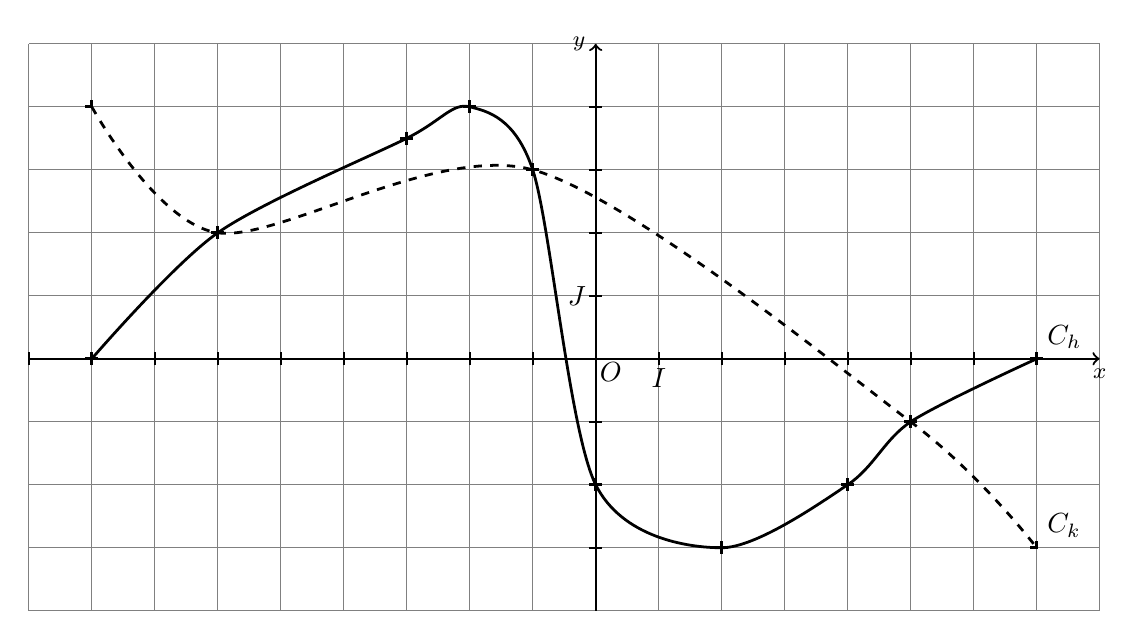
\begin{tikzpicture}[scale=0.8]
            \draw[gray] (-9,-4)grid(8,5);
            \draw[thick,->] (-9,0)--(8,0)node[below] {\footnotesize $x$};
            \draw[thick,->] (0,-4)--(0,5)node[left] {\footnotesize $y$};
            \coordinate (O) at (0,0); \draw (O) node[below right = -2pt] {$O$};
            \coordinate (I) at (1,0); \draw (I) node[below] {$I$}; \foreach \x in {-9,...,7}  \draw[line width=0.7pt] (\x,-0.1)--(\x,0.1);
            \coordinate (J) at (0,1); \draw (J) node[left] {$J$}; \foreach \x in {-3,...,4} \draw[line width=0.7pt] (-0.1,\x)--(0.1,\x);
            \draw[line width=1pt] plot[smooth=200,mark=+,mark options={scale =1.5}] coordinates{(-8,0)(-6,2)(-3,3.5)(-2,4)(-1,3)(0,-2)(2,-3)(4,-2)(5,-1)(7,0)} node[above right]{$\calig C_h$};
            \draw[dashed, line width=1pt] plot[smooth=200,mark=+,mark options={scale =1.5}] coordinates{(-8,4)(-6,2)(-1,3)(5,-1)(7,-3)} node[above right]{$\calig C_k$};
        \end{tikzpicture}
    \end{center}
\end{exoc}\[*\]


\end{document} 
